
% Start preamble
\documentclass[12pt,a4paper]{article}
\usepackage{geometry}
 \geometry{
 a4paper,
 total={170mm,257mm},
 left=20mm,
 top=20mm,
 }
\usepackage[utf8]{inputenc}
\usepackage[T1]{fontenc}
\usepackage[pdftex]{graphicx}
\graphicspath{{./}}
\usepackage{enumitem}
\usepackage{pdfpages}
\usepackage{hyperref}
\usepackage{tikz}
\usepackage{attachfile}
\usepackage{epstopdf}
\usepackage{array}
\usepackage{multirow}
\usepackage{multicol}
\usepackage{float}
%\usepackage[table]{xcolor,colorbl}
\setlength{\textwidth}{16cm}
\setlength{\oddsidemargin}{-0.5cm}
\setlength{\evensidemargin}{-0.5cm}
%\setlenght{\headsep}{0cm}
\setlength\parindent{0pt}
%\setlength{\extrarowheight}{3pt}
\usepackage{listings}
%\usepackage{xcolor}

\input{arduinoLanguage.tex}
%%%%%% Counting oppgaves %%%%%%
 \newcount\questnum \questnum=0
 \def\oppgave{
            \advance\questnum by 1
	    \ifthenelse{\questnum>0\AND \questnum<9}
	    {
                \vskip 1cm
		\textbf{Oppgave}\hskip 5pt\the\questnum \hfill \hfill(6p)
		\vskip 3pt
		\hrule
	\vskip 0.5cm}
	{
                \vskip 1cm
		\textbf{Oppgave}\hskip 5pt \the\questnum \hfill \hfill(12p)
		\vskip 3pt \hrule \vskip 0.5cm }

		}

% End preamble

\begin{document}
\title{PLS prøve 02}
\author{Faglærer: Fred-Olav Mosdal 90507684\\
Oppgave 1-8 gjøres på ark. Hjelpemidler: kalkulator. \\
Oppgave 9 gjøres på PC. Hjelpemidler: Alle ikke kommuniserende\\
Elektronisk del av prøve sendes på email til: \\
fred-olav.mosdal@skole.rogfk.no\\
Emne: Høstprøve}
\maketitle
\newpage
\vskip 2.5pt 

Prøven omhandler funksjonalitet rundt en tank for automatisk fylling av en tank. 
Du skal utvide funksjonaliteten til styringen for hver oppgave. Det
starter enkelt og blir vanskligere og vanskligere. 
\vskip 1cm
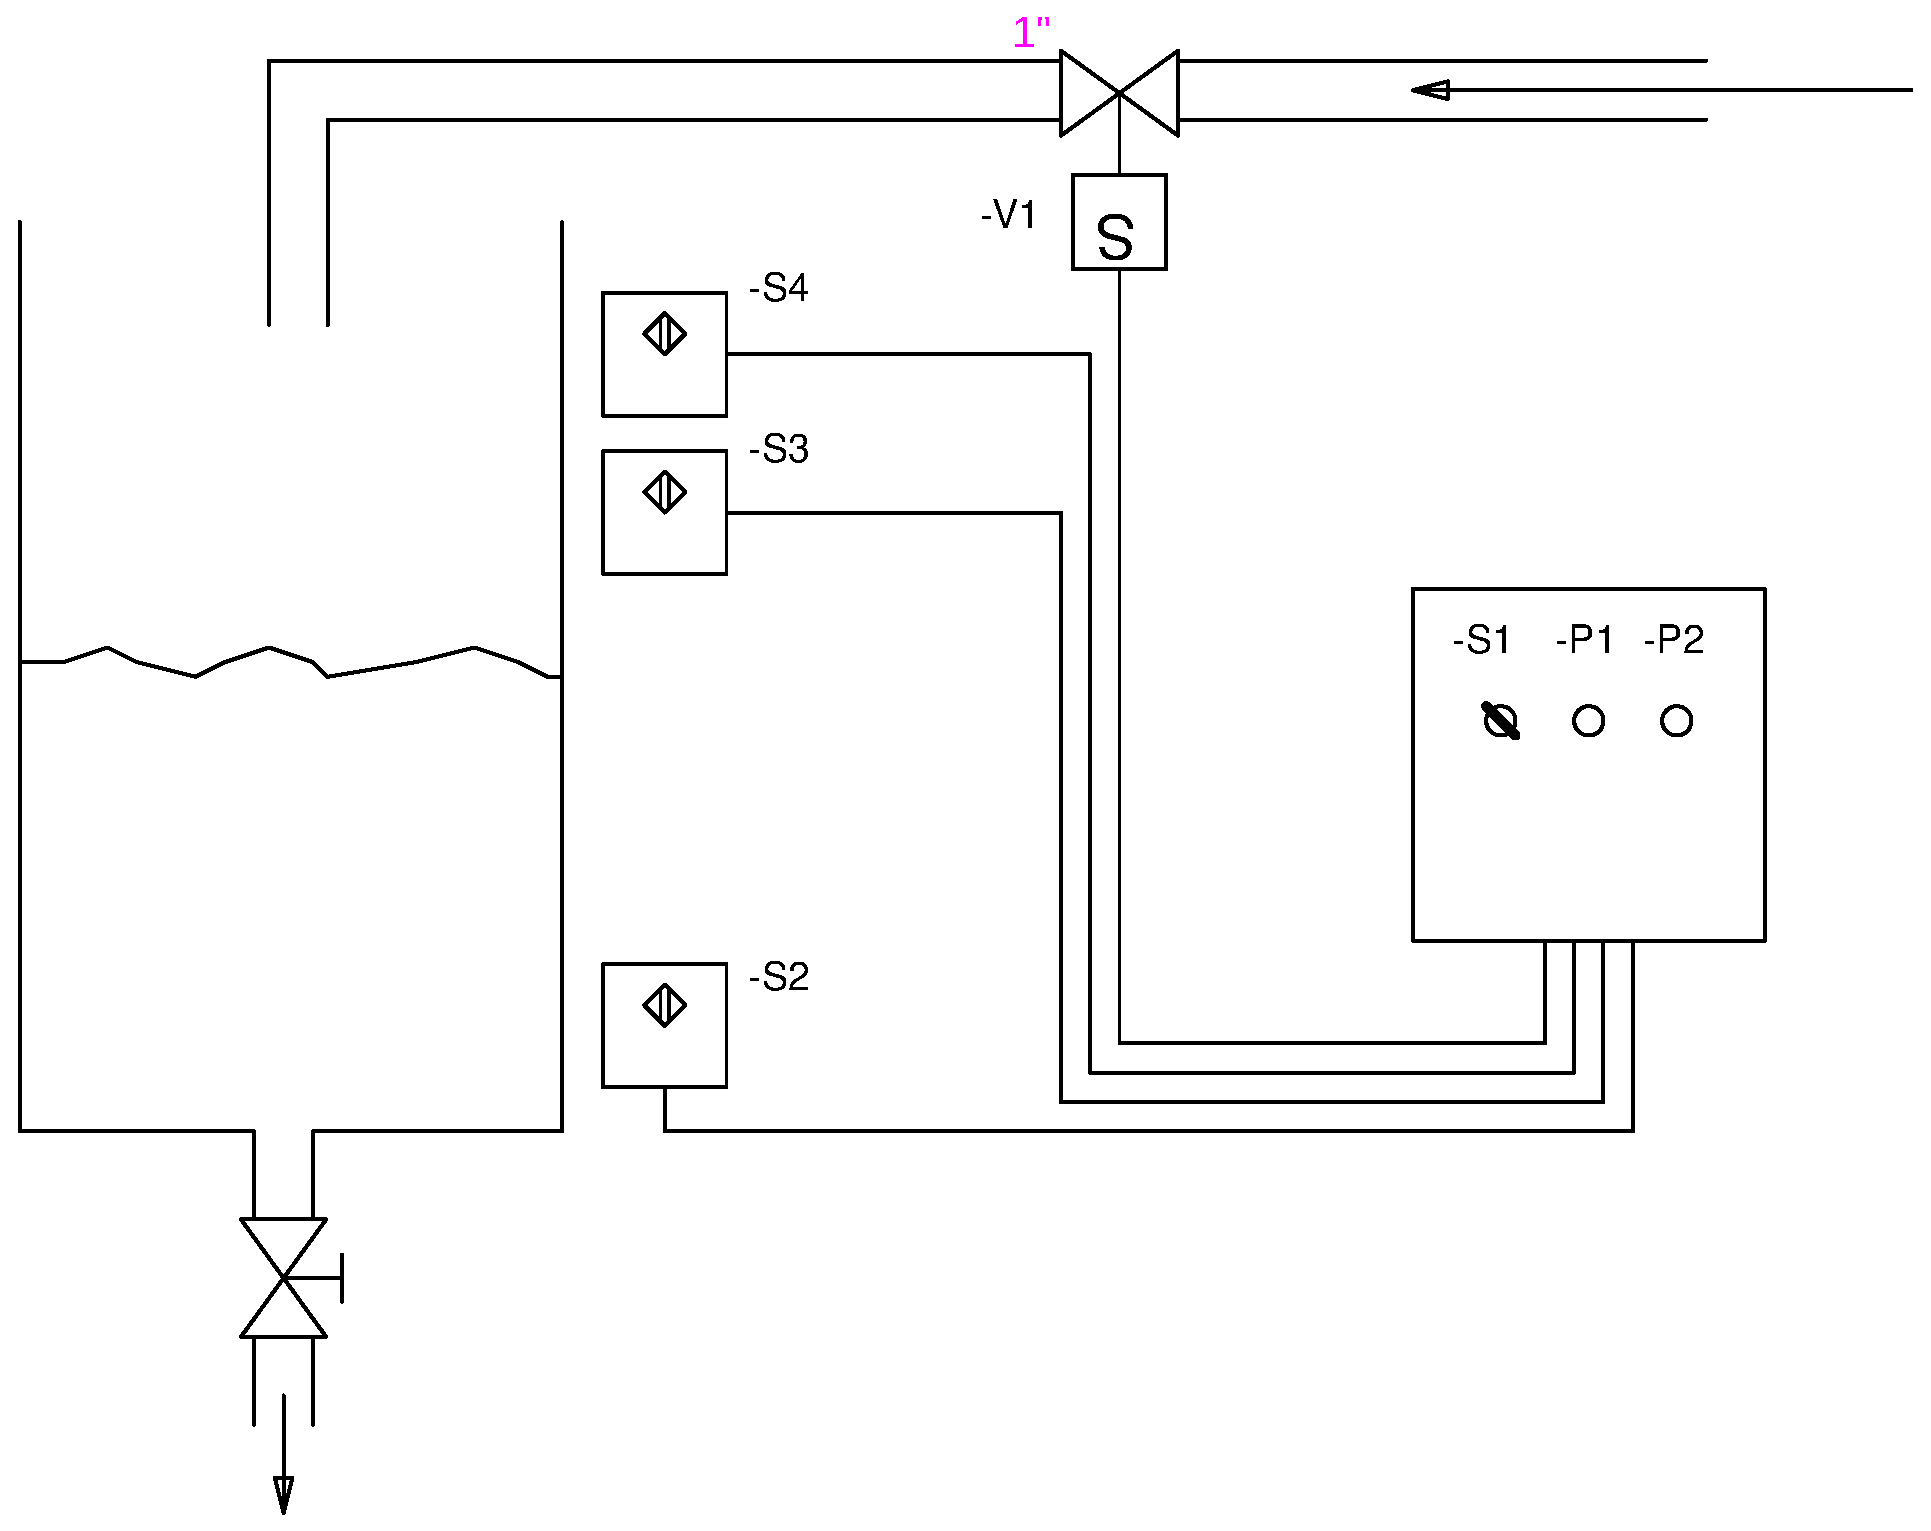
\includegraphics[width=1\textwidth]{aPLSProg02x01.eps}

\vskip 1cm
Det skal være skjermstyring som gør det lettere å test funksjonen. 
\vskip 10pt
\oppgave{}

Tanken på bildet skal fylles automatisk. Når nivået synker under posisjonen til -S2, aktiveres magnetventilen -V1, og tanken fylles opp. Når nivået kommer opp til -S3, kobler magnetventilen ut. 
\oppgave{}

Anlegget startes med venderen -S1, og signallampen -P1 angir at anlegget er aktivert (spenning på). 
\oppgave{}


Dersom nivået i tanken av en eller annen grunn (komponentsvikt e.l.) skulle stige opp til alarmgiveren -S4, aktiveres signallampen -P2 (og magnetventilen skal stenge). Den kapasitive giveren -S4 har en invertert utgang (NC) for på den måten oppnå en selvovervåkning av alarmkretsen (en komponentsvikt eller brudd i kabelen vil utløse alarmen). 
\oppgave{}


Når esken er full (10 deler), skal transportbåndet stoppe og det skal gis signal om at eske er full. Ved å trykke Ny Eske skal det være mulig å starte båndet på nytt. 
\oppgave{}


Om det ikke er registrert ny del på 15s skal transportbåndet stoppe og et varsellys aktiveres. Når en ser at det er nye deler klare, starer en bare båndet manuelt igjen. 
\oppgave{}


Legg til funksjonalitet slik at motorlampen blinker 1Hz under forsinket start. 
\oppgave{}
\newpage
\

\end{document}
